\documentclass{beamer}

\usepackage[utf8]{inputenc}
\input{../helper}
\usetikzlibrary{shapes.geometric}

\title{Introdução à Computação \\ árvores binárias de busca}
\author{Alexandre Rademaker}
\date{}

\begin{document}

\begin{frame}
 \maketitle
\end{frame}


\begin{frame}[allowframebreaks,fragile]{árvores}

  Uma árvore é um tipo de dados que representa um conjunto de nós
  conectados em uma estrutura hierárquica.

  Cada nó de uma árvore pode ser conectado a um número qualquer de
  \emph{filhos} - dependendo do tipo de árvore - mas apenas à um
  \emph{pai}. Um único nó, chamado \emph{raiz}, não tem pai.

  Isto siginifica que árvores não podem conter \emph{ciclos} e que
  cada nó pode ser considerado raiz de uma sub-árvore.

  Com isso, \emph{recursão} é uma técnica útil para travesia da
  árvore.

  \framebreak

  \begin{columns}
    \begin{column}{.4\textwidth}
      \begin{itemize}
      \item raiz
      \item folhas
      \item sub-árvores
      \item grau
      \item nível
      \item altura
      \end{itemize}
    \end{column}
    \begin{column}{.6\textwidth}
      \begin{center}
        
\includegraphics[width=.9\textwidth]{trees.png}
      \end{center}
    \end{column}
  \end{columns}
  
  \framebreak

  \emph{Árvores binárias} são um tipo de árvore onde cada nó pode
  conter até dois filhos.

  Quando a ordem dos filhos é relevante, chamamos de \emph{árvore
    ordenada}.

  Valores podem ser associados a cada nó na árvore ou, as vezes,
  apenas aos nós \emph{folhas} - nós que não tem filhos.

  \framebreak

  aplicações:

  \begin{itemize}
  \item sistema de arquivos dos sistemas operacionais
  \item DOM de páginas HTML e arquivos XML
  \item árvores de busca para armazenamento de dados de forma a
    permitir buscas eficientes.
  \item árvores sintáticas no processamento de linguagem natural.
  \end{itemize}

  \framebreak

  Um \emph{tipo abstrato de dados} pode ser representado de diferentes
  formas.

  Na memória, tipicamente nós são alocados dinamicamente com ponteiros
  para os filhos, pais, ou ambos, além dos dados associados ao nó.

  Se o número de filhos é variado, a cada nó podemos usar um array ou
  lista encadeada para armazenar ponteiros para os filhos.

  Também podemos representar a árvore com duas listas, uma para os nós
  e outra para as relações pai-filho (lista de adjacencias), ou um
  array onde os relacionamentos (pai-filho) são determinados pelas
  posições no array.

  \framebreak

  \begin{lstlisting}[style=code,language=lisp]
    '(2 (7 (2) (10) (6 (5) (11))) 
        (5 (9 (4))))
  \end{lstlisting}

  Se nossa implementação de lista encadeada permitisse que elementos
  da lista fossem de qualquer tipo, incluíndo listas\ldots

  também poderíamos implementar uma árvore como uma lista de listas,
  onde o primeiro elemento de cada sublista é a raiz da sub-árvore.

  Para saber \href{https://en.wikipedia.org/wiki/Tree_(data_structure)}{mais}!

\end{frame}


\begin{frame}[allowframebreaks, fragile]{árvores binárias de busca}

  Uma árvore binária de busca, também chamada de árvore binária
  ordenada, é uma árvore binária onde o valor de cada nó interno é
  maior que todos os valores na subárvore esquerda do respectivo nó e
  menor que as de sua subárvore direita.

  A complexidade de tempo das operações na árvore de busca binária é
  diretamente proporcional à altura da árvore.

  Buscas binárias podem ser facilmente implementadas em árvores
  binárias de busca.

  \framebreak

  
\includegraphics[width=.6\textwidth]{btree.png}
  
  \framebreak
  
  Em C, os nós precisam ser agora declarados com

  \begin{lstlisting}[style=normalc,caption=tree.c]
    typedef struct node {
      int key;
      struct node *left, *right;
    } t_node;
  \end{lstlisting}

  \framebreak

  Para inserir um novo elemento, uma função auxiliar que cria um novo
  nó:

  \begin{lstlisting}[style=normalc,caption=tree.c]
    t_node* new_node(int item) {
      t_node* t = malloc(sizeof(struct node));
      assert(t != NULL);
      t->key = item;
      t->left = t->right = NULL;
      return t;
    }
  \end{lstlisting}

  Notação \texttt{a = b = expressão}!

  \framebreak

  Agora a inserção, seja o nó corrente com valor V, devemos comparar
  com o valor X sendo inserido. Se X menor, movemos para a árvore à
  esquerda. Se X maior, para árvore da direita.

  \begin{lstlisting}[style=normalc,caption=tree.c]
    t_node* insert(t_node* node, int key) {
      if (node == NULL)
        return new_node(key);
      
      if (key < node->key)
        node->left = insert(node->left, key);
      else if (key > node->key)
        node->right = insert(node->right, key);
      
      return node;
    }
  \end{lstlisting}

  \framebreak

  
\includegraphics[width=.8\textwidth]{btree-insert.png}

  \framebreak

  Nós criados de forma dinâmica precisam ser liberados.

  \begin{lstlisting}[style=normalc, caption=tree.c]
    void free_tree(node *root) {
      if (root == NULL)
        return;

      free_tree(root->left);
      free_tree(root->right);
      free(root);
    }
  \end{lstlisting}

\end{frame}

\begin{frame}[allowframebreaks,fragile]{busca binária}

  Usando esta estrutura, podemos então realizar buscas\vspace{.5em}

  \begin{lstlisting}[style=normalc,caption=tree.c]
    bool binary_search(t_node *root, int n) {
      if (root == NULL)
        return false;
      else if (n < root->key)
        return binary_search(root->left, n);
      else if (n > root->key)
        return binary_search(root->right, n);
      return (n == root->key);
    }
  \end{lstlisting}

  \framebreak

  \begin{columns}
    \begin{column}{.5\textwidth}
      Mas temos que 'balancear' a árvore, para não terminar com uma
      estruta ineficiente.\vspace{1em}

      Em uma árvore balanceada, busca e inserção são $O(\log n)$, mas
      em uma árvore não balanceada, pode ser $O(n)$.
    \end{column}
    \begin{column}{.5\textwidth}
      \begin{center}
        
\includegraphics[width=.8\textwidth]{imbalanced_tree.png}
      \end{center}
    \end{column}
  \end{columns}

\end{frame}


\begin{frame}[allowframebreaks,fragile]{rebalanceamento ``em batch''}

  Uma primeira abordagem: depois de carregar todos os elementos,
  achatamos a árvore em um array ordenado (basta um \emph{inorder}) e
  reconstruímos tomando o elemento do meio como raiz, recursivamente.

  Custo $O(n)$, mas é uma operação ocasional. Para
  \texttt{sorted50000.txt} a altura cai de 50000 para
  $\lceil \log_2 50000 \rceil \approx 16$.

  \framebreak

  \begin{lstlisting}[style=normalc,caption=tree.c]
    int size(t_node* root) {
      if (root == NULL) return 0;
      return 1 + size(root->left) + size(root->right);
    }

    void to_array(t_node* root, t_node** arr, int* i) {
      if (root == NULL) return;
      to_array(root->left, arr, i);
      arr[(*i)++] = root;
      to_array(root->right, arr, i);
    }
  \end{lstlisting}

  \framebreak

  \begin{lstlisting}[style=normalc,caption=tree.c]
    t_node* from_sorted(t_node** arr, int lo, int hi) {
      if (lo > hi) return NULL;
      int mid = (lo + hi) / 2;
      t_node* root = arr[mid];
      root->left  = from_sorted(arr, lo, mid - 1);
      root->right = from_sorted(arr, mid + 1, hi);
      return root;
    }
  \end{lstlisting}

  \framebreak

  \begin{lstlisting}[style=normalc,caption=tree.c]
    t_node* balance(t_node* root) {
      int n = size(root);
      t_node** arr = malloc(n * sizeof(t_node*));
      int i = 0;
      to_array(root, arr, &i);
      t_node* novo = from_sorted(arr, 0, n - 1);
      free(arr);
      return novo;
    }
  \end{lstlisting}

  Observe que \texttt{to\_array} e \texttt{from\_sorted}
  \emph{reaproveitam} os mesmos nós; não há alocação de novos nós, só
  reorganização dos ponteiros.

\end{frame}


\begin{frame}[allowframebreaks,fragile]{AVL --- balanceamento a cada inserção}

  Outra abordagem: manter a árvore balanceada \emph{durante} as
  inserções. Cada \emph{insert} passa a custar $O(\log n)$ no pior
  caso, inclusive para entradas ordenadas.

  Cada nó passa a armazenar a sua altura. Definimos o \emph{fator de
    balanceamento} de um nó como a diferença entre as alturas das
  subárvores esquerda e direita. A árvore é dita AVL quando esse fator
  está em $\{-1, 0, +1\}$ para todo nó.

  \framebreak

  \begin{lstlisting}[style=normalc,caption=tree.c]
    typedef struct node {
      int key;
      int height;
      struct node *left, *right;
    } t_node;
  \end{lstlisting}

  O campo \texttt{height} é \emph{ignorado} pelas funções já vistas
  (\texttt{insert}, \texttt{height}, \texttt{binary\_search}). Ele
  passa a ser usado apenas pelas funções a seguir.

  \framebreak

  \begin{lstlisting}[style=normalc,caption=tree.c]
    int node_height(t_node* n) {
      return n == NULL ? 0 : n->height;
    }

    int balance_factor(t_node* n) {
      return node_height(n->left) - node_height(n->right);
    }

    void update_height(t_node* n) {
      int l = node_height(n->left);
      int r = node_height(n->right);
      n->height = 1 + (l > r ? l : r);
    }
  \end{lstlisting}

\end{frame}


\begin{frame}[allowframebreaks,fragile]{AVL --- rotações}

  Uma rotação reorganiza localmente três nós, preservando a propriedade
  de árvore binária de busca --- a sequência do \emph{inorder} não muda
  --- e podendo reduzir a altura local.

  \framebreak

  \begin{center}
    \begin{tikzpicture}[
        n/.style={circle, draw, minimum size=.65cm, inner sep=0pt},
        sub/.style={regular polygon, regular polygon sides=3, draw,
                    minimum size=.7cm, inner sep=0pt, font=\scriptsize},
        level distance=.85cm, sibling distance=1.2cm]

      \node[n] {y}
        child { node[n] {x}
          child { node[sub] {$T_1$} }
          child { node[sub] {$T_2$} } }
        child { node[sub] {$T_3$} };

      \node at (3.2,-1.4) {$\xrightarrow{\;\texttt{rotate\_right}(y)\;}$};

      \begin{scope}[xshift=6.4cm]
        \node[n] {x}
          child { node[sub] {$T_1$} }
          child { node[n] {y}
            child { node[sub] {$T_2$} }
            child { node[sub] {$T_3$} } };
      \end{scope}
    \end{tikzpicture}
  \end{center}

  \emph{Inorder} antes e depois: $T_1$, x, $T_2$, y, $T_3$ --- a
  propriedade de BST se preserva. \texttt{rotate\_left} é simétrica.

  \framebreak

  \begin{lstlisting}[style=normalc,caption=tree.c]
    t_node* rotate_right(t_node* y) {
      t_node* x = y->left;
      t_node* t = x->right;
      x->right = y;
      y->left  = t;
      update_height(y);
      update_height(x);
      return x;
    }
  \end{lstlisting}

  \framebreak

  \begin{lstlisting}[style=normalc,caption=tree.c]
    t_node* rotate_left(t_node* x) {
      t_node* y = x->right;
      t_node* t = y->left;
      y->left  = x;
      x->right = t;
      update_height(x);
      update_height(y);
      return y;
    }
  \end{lstlisting}

\end{frame}


\begin{frame}[allowframebreaks,fragile]{AVL --- inserção}

  Depois da inserção recursiva, atualizamos a altura do nó e
  verificamos o fator de balanceamento. Se ele sair do intervalo
  $[-1, +1]$, aplicamos uma ou duas rotações --- são quatro casos:
  \texttt{LL}, \texttt{RR}, \texttt{LR}, \texttt{RL}.

  Seja \texttt{z} o ancestral mais próximo do nó recém-inserido (em
  vermelho) cujo fator de balanceamento ficou fora de $[-1, +1]$, e
  \texttt{y} o filho de \texttt{z} no lado mais alto:

  \framebreak

  \begin{center}
    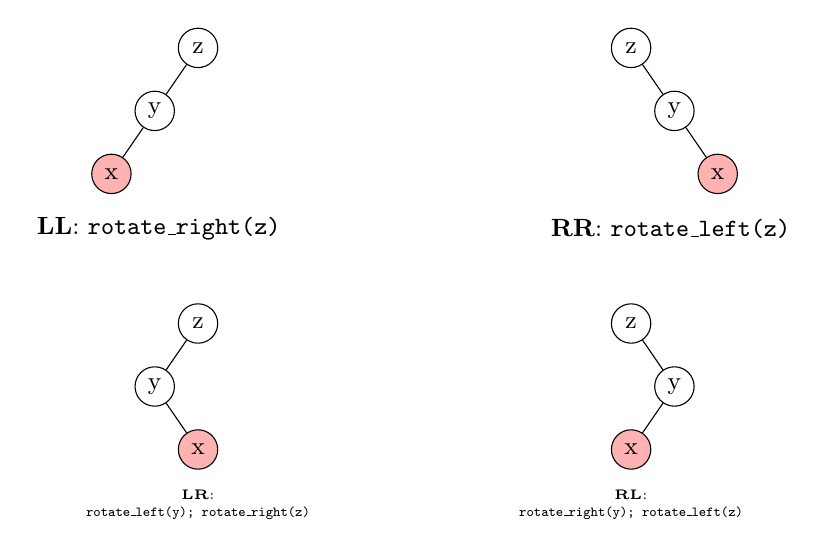
\begin{tikzpicture}[
        n/.style={circle, draw, minimum size=.5cm, inner sep=1pt, font=\small},
        nx/.style={n, fill=red!30}]

      % LL
      \node[n] (z0) at (0,0) {z};
      \node[n] (y0) at (-.55,-.8) {y};
      \node[nx] (x0) at (-1.1,-1.6) {x};
      \draw (z0) -- (y0) -- (x0);
      \node[font=\small] at (-.5,-2.3)
        {\textbf{LL}: \texttt{rotate\_right(z)}};

      % RR
      \begin{scope}[xshift=5.5cm]
        \node[n] (z1) at (0,0) {z};
        \node[n] (y1) at (.55,-.8) {y};
        \node[nx] (x1) at (1.1,-1.6) {x};
        \draw (z1) -- (y1) -- (x1);
        \node[font=\small] at (.5,-2.3)
          {\textbf{RR}: \texttt{rotate\_left(z)}};
      \end{scope}

      % LR
      \begin{scope}[yshift=-3.5cm]
        \node[n] (z2) at (0,0) {z};
        \node[n] (y2) at (-.55,-.8) {y};
        \node[nx] (x2) at (0,-1.6) {x};
        \draw (z2) -- (y2) -- (x2);
        \node[font=\tiny, align=center] at (0,-2.3)
          {\textbf{LR}:\\
           \texttt{rotate\_left(y); rotate\_right(z)}};
      \end{scope}

      % RL
      \begin{scope}[xshift=5.5cm, yshift=-3.5cm]
        \node[n] (z3) at (0,0) {z};
        \node[n] (y3) at (.55,-.8) {y};
        \node[nx] (x3) at (0,-1.6) {x};
        \draw (z3) -- (y3) -- (x3);
        \node[font=\tiny, align=center] at (0,-2.3)
          {\textbf{RL}:\\
           \texttt{rotate\_right(y); rotate\_left(z)}};
      \end{scope}
    \end{tikzpicture}
  \end{center}

  \framebreak

  \begin{lstlisting}[style=normalc,caption=tree.c]
    t_node* insert_avl(t_node* node, int key) {
      if (node == NULL) return new_node(key);

      if      (key < node->key)
        node->left  = insert_avl(node->left, key);
      else if (key > node->key)
        node->right = insert_avl(node->right, key);
      else return node;

      update_height(node);
      int bf = balance_factor(node);
  \end{lstlisting}

  \framebreak

  \begin{lstlisting}[style=normalc,caption=tree.c]
      // LL
      if (bf >  1 && key < node->left->key)
        return rotate_right(node);
      // RR
      if (bf < -1 && key > node->right->key)
        return rotate_left(node);
      // LR
      if (bf >  1 && key > node->left->key) {
        node->left = rotate_left(node->left);
        return rotate_right(node);
      }
      // RL
      if (bf < -1 && key < node->right->key) {
        node->right = rotate_right(node->right);
        return rotate_left(node);
      }

      return node;
    }
  \end{lstlisting}

  Em \texttt{main}, basta trocar \texttt{insert} por \texttt{insert\_avl}
  para que \texttt{sorted50000.txt} caia da altura 50000 para
  $\approx 16$.

\end{frame}


\begin{frame}[allowframebreaks,fragile]{AVL --- exemplo}

  Inserindo a sequência $1, 2, 3, 4, 5$ em uma AVL inicialmente vazia.
  Em \textcolor{red}{vermelho}, o nó recém-inserido; em
  \textcolor{cyan!70!black}{azul}, o ancestral onde
  $\textrm{bf} \notin [-1, +1]$ --- ponto de rotação.

  \framebreak

  Inserções $1$, $2$ e $3$:

  \begin{center}
    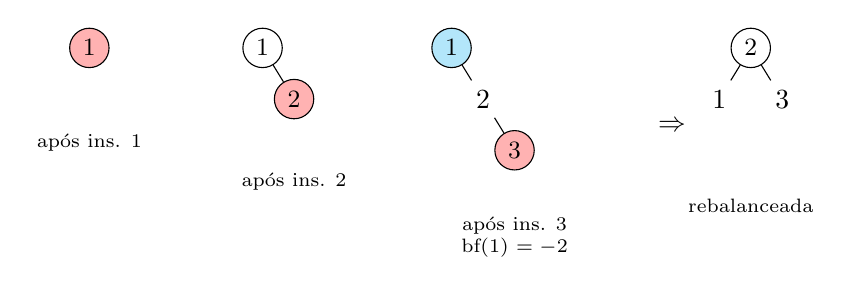
\begin{tikzpicture}[
        n/.style={circle, draw, minimum size=.5cm, inner sep=1pt, font=\small},
        new/.style={n, fill=red!30},
        pivot/.style={n, fill=cyan!30},
        level distance=.65cm, sibling distance=.8cm,
        lbl/.style={font=\scriptsize}]

      % t1: insert 1
      \node[new] {1};
      \node[lbl] at (0,-1.2) {após ins. 1};

      % t2: insert 2
      \begin{scope}[xshift=2.2cm]
        \node[n] {1}
          child[missing] {}
          child { node[new] {2} };
        \node[lbl] at (.4,-1.7) {após ins. 2};
      \end{scope}

      % t3a: insert 3 (chain, pivot at 1)
      \begin{scope}[xshift=4.6cm]
        \node[pivot] {1}
          child[missing] {}
          child { node {2}
            child[missing] {}
            child { node[new] {3} } };
        \node[lbl, align=center] at (.8,-2.4)
          {após ins. 3\\bf(1) $= -2$};
      \end{scope}

      \node at (7.4,-1) {$\Rightarrow$};

      % t3b: after rotation
      \begin{scope}[xshift=8.4cm]
        \node[n] {2}
          child { node {1} }
          child { node {3} };
        \node[lbl] at (0,-2) {rebalanceada};
      \end{scope}
    \end{tikzpicture}
  \end{center}

  \framebreak

  Continuando com $4$ e $5$:

  \begin{center}
    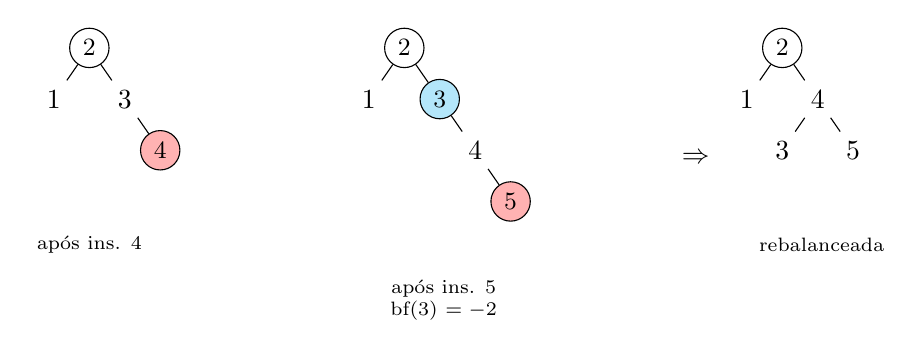
\begin{tikzpicture}[
        n/.style={circle, draw, minimum size=.5cm, inner sep=1pt, font=\small},
        new/.style={n, fill=red!30},
        pivot/.style={n, fill=cyan!30},
        level distance=.65cm, sibling distance=.9cm,
        lbl/.style={font=\scriptsize}]

      % t4: insert 4
      \node[n] {2}
        child { node {1} }
        child { node {3}
          child[missing] {}
          child { node[new] {4} } };
      \node[lbl] at (0,-2.5) {após ins. 4};

      % t5a: insert 5 (pivot at 3)
      \begin{scope}[xshift=4cm]
        \node[n] {2}
          child { node {1} }
          child { node[pivot] {3}
            child[missing] {}
            child { node {4}
              child[missing] {}
              child { node[new] {5} } } };
        \node[lbl, align=center] at (.5,-3.2)
          {após ins. 5\\bf(3) $= -2$};
      \end{scope}

      \node at (7.7,-1.4) {$\Rightarrow$};

      % t5b: after rotation
      \begin{scope}[xshift=8.8cm]
        \node[n] {2}
          child { node {1} }
          child { node {4}
            child { node {3} }
            child { node {5} } };
        \node[lbl] at (.5,-2.5) {rebalanceada};
      \end{scope}
    \end{tikzpicture}
  \end{center}

  \framebreak

  Para a sequência ordenada $1, 2, \ldots, n$, a árvore AVL termina
  com altura $\lceil \log_2 n \rceil + 1$ em vez de $n$.

  \vspace{1em}

  Animações interativas e detalhes adicionais:
  \href{https://en.wikipedia.org/wiki/AVL_tree}{en.wikipedia.org/wiki/AVL\_tree}
  (Wikipedia traz figuras CC-BY-SA das rotações e dos quatro casos, além
  de provas de complexidade).

\end{frame}


\end{document}

%%% Local Variables:
%%% mode: latex
%%% TeX-master: t
%%% End:
